\documentclass[11pt,a4paper]{report}
\usepackage[textwidth=37em,vmargin=30mm]{geometry}
\usepackage{calc,xunicode,amsmath,amssymb,paralist,enumitem,tabu,booktabs,datetime2,xeCJK,xeCJKfntef,listings}
\usepackage{tocloft,fancyhdr,tcolorbox,xcolor,graphicx,eso-pic,xltxtra,xelatexemoji}

\newcommand{\envyear}[0]{2025}
\newcommand{\envdatestr}[0]{2025-03-17}
\newcommand{\envfinaldir}[0]{webdb/2025/20250317/final}

\usepackage[hidelinks]{hyperref}
\hypersetup{
    colorlinks=false,
    pdfpagemode=FullScreen,
    pdftitle={Web Digest - \envdatestr}
}

\setlength{\cftbeforechapskip}{10pt}
\renewcommand{\cftchapfont}{\rmfamily\bfseries\large\raggedright}
\setlength{\cftbeforesecskip}{2pt}
\renewcommand{\cftsecfont}{\sffamily\small\raggedright}

\setdefaultleftmargin{2em}{2em}{1em}{1em}{1em}{1em}

\usepackage{xeCJK,xeCJKfntef}
\xeCJKsetup{PunctStyle=plain,RubberPunctSkip=false,CJKglue=\strut\hskip 0pt plus 0.1em minus 0.05em,CJKecglue=\strut\hskip 0.22em plus 0.2em}
\XeTeXlinebreaklocale "zh"
\XeTeXlinebreakskip = 0pt


\setmainfont{Brygada 1918}
\setromanfont{Brygada 1918}
\setsansfont{IBM Plex Sans}
\setmonofont{JetBrains Mono NL}
\setCJKmainfont{Noto Serif CJK SC}
\setCJKromanfont{Noto Serif CJK SC}
\setCJKsansfont{Noto Sans CJK SC}
\setCJKmonofont{Noto Sans CJK SC}

\setlength{\parindent}{0pt}
\setlength{\parskip}{8pt}
\linespread{1.15}

\lstset{
	basicstyle=\ttfamily\footnotesize,
	numbersep=5pt,
	backgroundcolor=\color{black!5},
	showspaces=false,
	showstringspaces=false,
	showtabs=false,
	tabsize=2,
	captionpos=b,
	breaklines=true,
	breakatwhitespace=true,
	breakautoindent=true,
	linewidth=\textwidth
}






\newcommand{\coverpic}[2]{
    % argv: itemurl, authorname
    Cover photo by #2~~(\href{#1}{#1})
}
\newcommand{\makeheader}[0]{
    \begin{titlepage}
        % \newgeometry{hmargin=15mm,tmargin=21mm,bmargin=12mm}
        \begin{center}
            
            \rmfamily\scshape
            \fontspec{BaskervilleF}
            \fontspec{Old Standard}
            \fontsize{59pt}{70pt}\selectfont
            WEB\hfill DIGEST
            
            \vfill
            % \vskip 30pt
            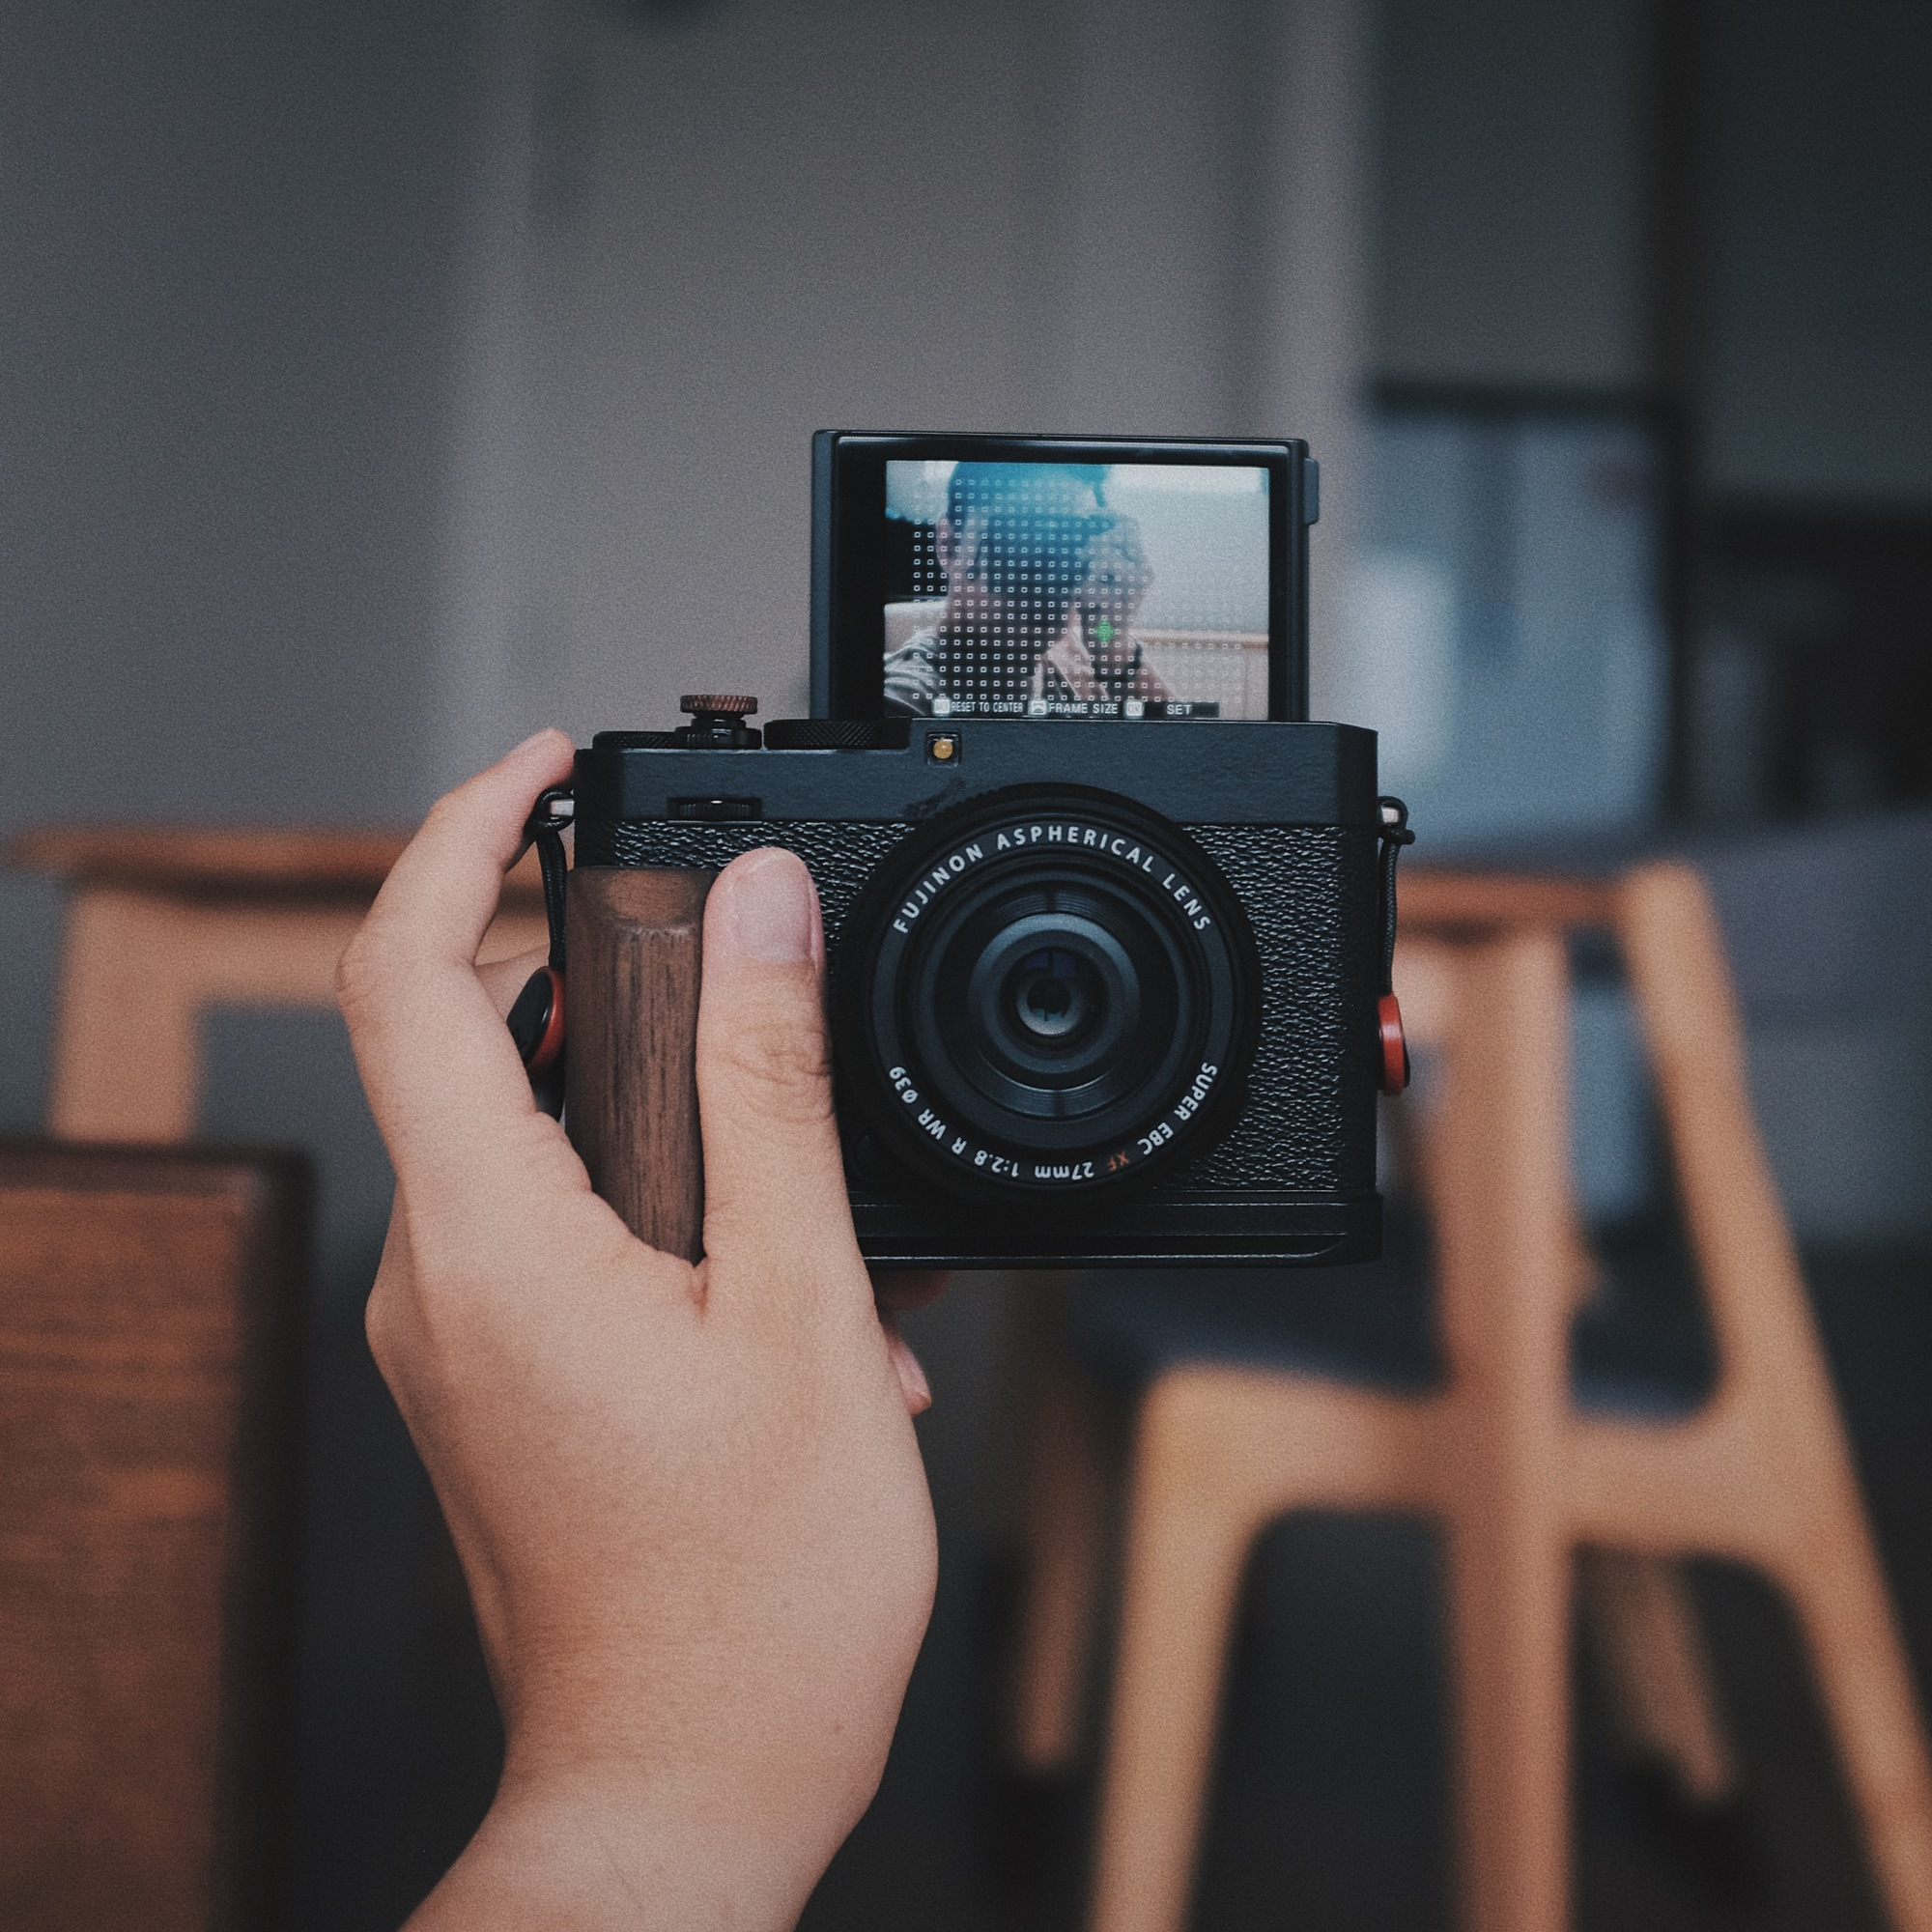
\includegraphics[width=\linewidth]{\envfinaldir/coverpic-prod.jpg}\par
            % \vskip 30pt
            \vfill

            \normalsize\rmfamily\scshape
            \copyright{} The Web Digest Project \hfill\large \envdatestr
        \end{center}
    \end{titlepage}
    % \restoregeometry
}
\newcommand{\simplehref}[1]{%
    \textcolor{blue!80!green}{\href{#1}{#1}}%
}
\renewcommand{\contentsname}{\center\Huge\sffamily\bfseries Contents\par\vskip 20pt}
\newcounter{ipartcounter}
\setcounter{ipartcounter}{0}
\newcommand{\ipart}[1]{
    % \vskip 20pt
    \clearpage
    \stepcounter{ipartcounter}
    \phantomsection
    \addcontentsline{toc}{chapter}{#1}
    % \begin{center}
    %     \Huge
    %     \sffamily\bfseries
    %     #1
    % \end{center}
    % \vskip 20pt plus 7pt
}
\newcounter{ichaptercounter}
\setcounter{ichaptercounter}{0}
\newcommand{\ichapter}[1]{
    % \vskip 20pt
    \clearpage
    \stepcounter{ichaptercounter}
    \phantomsection
    \addcontentsline{toc}{section}{\numberline{\arabic{ichaptercounter}}#1}
    \begin{center}
        \Huge
        \sffamily\bfseries
        #1
    \end{center}
    \vskip 20pt plus 7pt
}
\newcommand{\entrytitlefont}[1]{\subsection*{\raggedright\Large\sffamily\bfseries#1}}
\newcommand{\entryitemGeneric}[2]{
    % argv: title, url
    \parbox{\linewidth}{
        \entrytitlefont{#1}\par\vskip 5pt
        \footnotesize\ttfamily\mdseries
        \simplehref{#2}
    }\vskip 11pt plus 11pt minus 1pt
}
\newcommand{\entryitemGithub}[3]{
    % argv: title, url, desc
    \parbox{\linewidth}{
        \entrytitlefont{#1}\par\vskip 5pt
        \footnotesize\ttfamily\mdseries
        \simplehref{#2}\par\vskip 5pt
        \small\rmfamily\mdseries#3
    }\vskip 11pt plus 11pt minus 1pt
}
\newcommand{\entryitemAp}[3]{
    % argv: title, url, desc
    \parbox{\linewidth}{
        \entrytitlefont{#1}\par\vskip 5pt
        \footnotesize\ttfamily\mdseries
        \simplehref{#2}\par\vskip 5pt
        \small\rmfamily\mdseries#3
    }\vskip 11pt plus 11pt minus 1pt
}
\newcommand{\entryitemHackernews}[3]{
    % argv: title, hnurl, rawurl
    % \parbox{\linewidth}{
    %     \entrytitlefont{#1}\par\vskip 5pt
    %     \footnotesize\ttfamily\mdseries
    %     \simplehref{#3}\par
    %     \textcolor{black!50}{\href{#2}{#2}}
    % }\vskip 11pt plus 11pt minus 1pt
    \begin{minipage}{\linewidth}
            \entrytitlefont{#1}\par\vskip 5pt
            \footnotesize\ttfamily\mdseries
            \simplehref{#3}\par
            \textcolor{black!50}{\href{#2}{#2}}
    \end{minipage}\par\vskip 11pt plus 11pt minus 1pt
}







\begin{document}

\makeheader

\tableofcontents\clearpage




\ipart{Developers}
\ichapter{Hacker News}
\entryitemTwoLinks{Tesla drives into Wile E. Coyote fake road wall in camera vs. Lidar test}{https://news.ycombinator.com/item?id=43382230}{https://electrek.co/2025/03/16/tesla-autopilot-drives-into-wall-camera-vs-lidar-test/}

\entryitemTwoLinks{Military grade sonic weapon is used against protesters in Serbia}{https://news.ycombinator.com/item?id=43382093}{https://twitter.com/nexta\_tv/status/1901244199220982213}

\entryitemTwoLinks{Zlib-rs is faster than C}{https://news.ycombinator.com/item?id=43381512}{https://trifectatech.org/blog/zlib-rs-is-faster-than-c/}

\entryitemTwoLinks{AI Is Making Developers Dumb}{https://news.ycombinator.com/item?id=43381215}{https://eli.cx/blog/ai-is-making-developers-dumb}

\entryitemTwoLinks{Our interfaces have lost their senses}{https://news.ycombinator.com/item?id=43380930}{https://wattenberger.com/thoughts/our-interfaces-have-lost-their-senses}

\entryitemTwoLinks{"Wait, not like that": Free and open access in the age of generative AI}{https://news.ycombinator.com/item?id=43380617}{https://www.citationneeded.news/free-and-open-access-in-the-age-of-generative-ai/}

\entryitemTwoLinks{DiceDB}{https://news.ycombinator.com/item?id=43379262}{https://dicedb.io/}

\entryitemTwoLinks{Learn You Some Erlang for Great Good (2013)}{https://news.ycombinator.com/item?id=43378415}{https://learnyousomeerlang.com/content}

\entryitemTwoLinks{Big LLMs weights are a piece of history}{https://news.ycombinator.com/item?id=43378401}{https://antirez.com/news/147}

\entryitemTwoLinks{The good times in tech are over}{https://news.ycombinator.com/item?id=43378321}{https://www.seangoedecke.com/good-times-are-over/}

\entryitemTwoLinks{Docs – Open source alternative to Notion or Outline}{https://news.ycombinator.com/item?id=43378239}{https://github.com/suitenumerique/docs}

\entryitemTwoLinks{GPT 4.5 level for 1\% of the price}{https://news.ycombinator.com/item?id=43377962}{https://twitter.com/Baidu\_Inc/status/1901089355890036897}

\entryitemTwoLinks{Lynx is the oldest web browser still being maintained}{https://news.ycombinator.com/item?id=43377829}{https://news.ycombinator.com/item?id=43377829}

\entryitemTwoLinks{Show HN: My high school team's space probe}{https://news.ycombinator.com/item?id=43377690}{https://drive.google.com/file/d/1\_9V6lBTIfDsPdKCohQBc5Ed5UzDbnsrI/view?usp=sharing}

\entryitemTwoLinks{Generate impressive-looking terminal output, look busy when stakeholders walk by}{https://news.ycombinator.com/item?id=43376824}{https://github.com/giacomo-b/rust-stakeholder}

\entryitemTwoLinks{Cloudflare asks browser devs to sign insane NDAs before fixing browser blocking}{https://news.ycombinator.com/item?id=43376064}{https://forum.palemoon.org/viewtopic.php?t=32127}

\entryitemTwoLinks{Apple's long-lost hidden recovery partition from 1994 has been found}{https://news.ycombinator.com/item?id=43376033}{https://www.downtowndougbrown.com/2025/03/apples-long-lost-hidden-recovery-partition-from-1994-has-been-found/}

\entryitemTwoLinks{Career Advice in 2025}{https://news.ycombinator.com/item?id=43375923}{https://lethain.com/career-advice-2025/}

\entryitemTwoLinks{ESP32 WiFi Superstitions}{https://news.ycombinator.com/item?id=43375780}{https://supakeen.com/weblog/esp32-wifi-superstitions/}

\entryitemTwoLinks{Sign in as anyone: Bypassing SAML SSO authentication with parser differentials}{https://news.ycombinator.com/item?id=43374519}{https://github.blog/security/sign-in-as-anyone-bypassing-saml-sso-authentication-with-parser-differentials/}\ichapter{Phoronix}
\entryitemGeneric{\hskip 0pt{}Linux 6.14-rc7 Released With v6.14 Final Expected Next Weekend}{https://www.phoronix.com/news/Linux-6.14-rc7-Released}

\entryitemGeneric{\hskip 0pt{}DXVK-NVAPI 0.9 Brings New Features For NVIDIA GPUs With Valve's Steam Play}{https://www.phoronix.com/news/DXVK-NVAPI-0.9}

\entryitemGeneric{\hskip 0pt{}Arm Changing Linux Default To Costly "KPTI" Mitigation For Some Newer CPUs}{https://www.phoronix.com/news/Arm-Linux-CVE-2024-7881-KPTI}

\entryitemGeneric{\hskip 0pt{}Huawei Matebook E Go Laptops To Be Better Supported With Linux 6.15}{https://www.phoronix.com/news/Huawei-Matebook-E-Go-EC-Linux}

\entryitemGeneric{\hskip 0pt{}Linux 6.14-rc7 To Support A Few More Gaming Controllers}{https://www.phoronix.com/news/Linux-6.14-rc7-More-Controllers}

\entryitemGeneric{\hskip 0pt{}One Line Of Code Optimizes F2FS Performance For Small Multi-Threaded Writes}{https://www.phoronix.com/news/F2FS-Optimize-MT-Small-Writes}

\entryitemGeneric{\hskip 0pt{}Linux Kernel's Rust Support Being Expanded To HID Drivers}{https://www.phoronix.com/news/Linux-Rust-HID-Drivers-Patches}

\entryitemGeneric{\hskip 0pt{}Debian 12.10 Released With More Bugs Fixed \& Security Updates}{https://www.phoronix.com/news/Debian-12.10-Released}

\entryitemGeneric{\hskip 0pt{}Paid XR Desktop For GNOME "Breezy Desktop" In Open Beta With Multi-Display Support}{https://www.phoronix.com/news/GNOME-This-Week-Breezy}\ichapter{Dribbble}
\entryitemGeneric{\hskip 0pt{}Abstract S Logo Design // For Sale}{https://dribbble.com/shots/25764643-Abstract-S-Logo-Design-For-Sale}

\entryitemGeneric{\hskip 0pt{}Triceratops}{https://dribbble.com/shots/25761010-Triceratops}

\entryitemGeneric{\hskip 0pt{}Tab Bar Animation}{https://dribbble.com/shots/25760227-Tab-Bar-Animation}

\entryitemGeneric{\hskip 0pt{}Chief Logo Design Process}{https://dribbble.com/shots/25759736-Chief-Logo-Design-Process}

\entryitemGeneric{\hskip 0pt{}Carbon Solutions B2B Dashboard Design}{https://dribbble.com/shots/25681782-Carbon-Solutions-B2B-Dashboard-Design}

\entryitemGeneric{\hskip 0pt{}Logowave Awards Entry from Lepisov Branding}{https://dribbble.com/shots/25755190-Logowave-Awards-Entry-from-Lepisov-Branding}

\entryitemGeneric{\hskip 0pt{}Bir-D / D.Bird}{https://dribbble.com/shots/25757221-Bir-D-D-Bird}

\entryitemGeneric{\hskip 0pt{}Flare - Logo Design 🚀}{https://dribbble.com/shots/25754585-Flare-Logo-Design}

\entryitemGeneric{\hskip 0pt{}Squid Book}{https://dribbble.com/shots/25756273-Squid-Book}

\entryitemGeneric{\hskip 0pt{}Order detail dashboard}{https://dribbble.com/shots/25748173-Order-detail-dashboard}

\entryitemGeneric{\hskip 0pt{}Pricing Plan Web Page Design}{https://dribbble.com/shots/25755045-Pricing-Plan-Web-Page-Design}

\entryitemGeneric{\hskip 0pt{}Fishing Tournament Logo}{https://dribbble.com/shots/25750107-Fishing-Tournament-Logo}

\entryitemGeneric{\hskip 0pt{}Triceratops}{https://dribbble.com/shots/25749787-Triceratops}

\entryitemGeneric{\hskip 0pt{}Lamar® 21°}{https://dribbble.com/shots/25750164-Lamar-21}

\entryitemGeneric{\hskip 0pt{}Sergeant Scooper}{https://dribbble.com/shots/25749566-Sergeant-Scooper}

\entryitemGeneric{\hskip 0pt{}Atoms - Logo Concepts}{https://dribbble.com/shots/25749091-Atoms-Logo-Concepts}

\entryitemGeneric{\hskip 0pt{}Line Icons}{https://dribbble.com/shots/25749882-Line-Icons}

\entryitemGeneric{\hskip 0pt{}Logo For Designed.supply}{https://dribbble.com/shots/25748434-Logo-For-Designed-supply}

\entryitemGeneric{\hskip 0pt{}Logo Database (V7) 2024—25}{https://dribbble.com/shots/25743610-Logo-Database-V7-2024-25}

\entryitemGeneric{\hskip 0pt{}Codila Studio}{https://dribbble.com/shots/25749456-Codila-Studio}

\entryitemGeneric{\hskip 0pt{}Emergency App Concept Design}{https://dribbble.com/shots/25711688-Emergency-App-Concept-Design}

\entryitemGeneric{\hskip 0pt{}Crystal // Website}{https://dribbble.com/shots/25742820-Crystal-Website}

\entryitemGeneric{\hskip 0pt{}Sway}{https://dribbble.com/shots/25744097-Sway}

\entryitemGeneric{\hskip 0pt{}Partify}{https://dribbble.com/shots/25040893-Partify}


\ipart{Developers~~~~(zh-Hans)}
\ichapter{Solidot}
\entryitemGeneric{\hskip 0pt{}开源中国停止招募接收方、再次决定关闭スラド}{https://www.solidot.org/story?sid=80799}

\entryitemGeneric{\hskip 0pt{}空间站太干净不利于宇航员健康}{https://www.solidot.org/story?sid=80798}

\entryitemGeneric{\hskip 0pt{}回顾 Firefox 的分支}{https://www.solidot.org/story?sid=80797}

\entryitemGeneric{\hskip 0pt{}NASA、耶鲁和斯坦福的科学家考虑``科学流放''}{https://www.solidot.org/story?sid=80796}

\entryitemGeneric{\hskip 0pt{}超新星爆发可能导致了至少两次地球大规模灭绝事件}{https://www.solidot.org/story?sid=80795}

\entryitemGeneric{\hskip 0pt{}铁缺乏症的全球挑战}{https://www.solidot.org/story?sid=80794}

\entryitemGeneric{\hskip 0pt{}DeepSeek 在中国已经无处不在}{https://www.solidot.org/story?sid=80793}

\entryitemGeneric{\hskip 0pt{}黄金价格首次突破每盎司 3000 美元}{https://www.solidot.org/story?sid=80792}

\entryitemGeneric{\hskip 0pt{}玩家 2024 年在 Steam Deck 上的游戏时间比 2023 年增长 64\%}{https://www.solidot.org/story?sid=80791}

\entryitemGeneric{\hskip 0pt{}OpenAI 希望使用版权材料训练 AI 属于合理使用}{https://www.solidot.org/story?sid=80790}

\entryitemGeneric{\hskip 0pt{}澳大利亚男子在安装钛合金人造心脏后生存了 100 天}{https://www.solidot.org/story?sid=80789}

\entryitemGeneric{\hskip 0pt{}微软称 Windows 最近的一个更新会导致 USB 打印机打印随机文本}{https://www.solidot.org/story?sid=80788}

\entryitemGeneric{\hskip 0pt{}中生代哺乳动物有着深色皮毛}{https://www.solidot.org/story?sid=80787}\ichapter{V2EX}
\entryitemGeneric{\hskip 0pt{}[Local LLM] 如何估算一个大模型需要用到什么性能配置的硬件?}{https://www.v2ex.com/t/1118897}

\entryitemGeneric{\hskip 0pt{}[Digg] Digg Reboot}{https://www.v2ex.com/t/1118896}

\entryitemGeneric{\hskip 0pt{}[问与答] W11 的 左侧 小组件/磁贴 有办法完全关闭吗? 最好禁止运行}{https://www.v2ex.com/t/1118895}

\entryitemGeneric{\hskip 0pt{}[程序员] 后端如何线性的提升自己的开发能力,或者学习到一些最佳实践}{https://www.v2ex.com/t/1118894}

\entryitemGeneric{\hskip 0pt{}[分享创造] 鉴于 AI 编程越来越强大和流行,``程序员''越来越多,需求不够用了。我开发了一个分析全网用户需求的网站}{https://www.v2ex.com/t/1118893}

\entryitemGeneric{\hskip 0pt{}[Apple] iOS 上有啥比较好用的 RSS 阅读器嘛?}{https://www.v2ex.com/t/1118892}

\entryitemGeneric{\hskip 0pt{}[问与答] 求个给孩子讲题的 ai,求推荐,不知道豆包行么?}{https://www.v2ex.com/t/1118891}

\entryitemGeneric{\hskip 0pt{}[Python] 聊一个最近在做的 post-mortem debugging tool 吧}{https://www.v2ex.com/t/1118890}

\entryitemGeneric{\hskip 0pt{}[分享创造] 还有哪些场景是专业 Agent 的机会?}{https://www.v2ex.com/t/1118889}

\entryitemGeneric{\hskip 0pt{}[问与答] 从阿里云中国无障碍直连外网的方案有哪些?}{https://www.v2ex.com/t/1118888}

\entryitemGeneric{\hskip 0pt{}[酷工作] 星际动能 2025 年招聘启事(人工智能预测业务)}{https://www.v2ex.com/t/1118886}

\entryitemGeneric{\hskip 0pt{}[Apple] 损失几百万!苹果开发者账号被盗后,苹果不给找回}{https://www.v2ex.com/t/1118885}

\entryitemGeneric{\hskip 0pt{}[OpenWrt] 周末闲着没事使用 immortalwrt-imagebuilder 编译了 24.10 的版本刷了}{https://www.v2ex.com/t/1118884}

\entryitemGeneric{\hskip 0pt{}[问与答] 出租房 2 千预算的电视怎么选?}{https://www.v2ex.com/t/1118883}

\entryitemGeneric{\hskip 0pt{}[Google] Google 要让所有 Google Assistant 用户升级为 Google Gemini,香港用户怎么办?}{https://www.v2ex.com/t/1118882}

\entryitemGeneric{\hskip 0pt{}[求职] 7 年经验 Java 求职远程工作岗位, Web3 做过 SocialFi、CEX(钱包/现货撮合/行情 K 线)、NFT 合集,传统行业做过商业航天、SCRM 系统}{https://www.v2ex.com/t/1118881}

\entryitemGeneric{\hskip 0pt{}[问与答] 彩色激光一体机求推荐}{https://www.v2ex.com/t/1118880}

\entryitemGeneric{\hskip 0pt{}[北京] 北京姚家园二居室转租}{https://www.v2ex.com/t/1118878}

\entryitemGeneric{\hskip 0pt{}[问与答] 请问目前什么节点能使用 Talkatone?}{https://www.v2ex.com/t/1118877}

\entryitemGeneric{\hskip 0pt{}[问与答] 关于 wordpress 开发有点转不过来弯了}{https://www.v2ex.com/t/1118876}

\entryitemGeneric{\hskip 0pt{}[macOS] 请问下大家 macOS 下的 App 在同一台机的两个不用的用户上,需要双份激活码?}{https://www.v2ex.com/t/1118875}

\entryitemGeneric{\hskip 0pt{}[分享创造] 闲鱼智能回复助手—我把闲鱼变成了 agent 发布平台}{https://www.v2ex.com/t/1118874}

\entryitemGeneric{\hskip 0pt{}[程序员] AI 编程是否会带来强类型语言的普及? AI 写的 JS,如果是冷门一点的库经常弄错参数, IDE 没报错运行也不一定能发现}{https://www.v2ex.com/t/1118871}

\entryitemGeneric{\hskip 0pt{}[远程工作] 招高级计算机视觉工程师(Senior Computer Vision Engineer)}{https://www.v2ex.com/t/1118868}

\entryitemGeneric{\hskip 0pt{}[Go 编程语言] 现在搞 p2p 很简单了}{https://www.v2ex.com/t/1118867}

\entryitemGeneric{\hskip 0pt{}[问与答] 有什么好用的 png 转 svg 的工具或网站推荐?}{https://www.v2ex.com/t/1118866}

\entryitemGeneric{\hskip 0pt{}[macOS] chrome 和 edge 可以科学上网,但是 safari 却不可以}{https://www.v2ex.com/t/1118865}

\entryitemGeneric{\hskip 0pt{}[问与答] tailscale 和 frp 的显著区别是什么?}{https://www.v2ex.com/t/1118863}

\entryitemGeneric{\hskip 0pt{}[职场话题] 华为 OD 求前辈指教:成都事件 HC 暂停是否影响已谈薪的 offer?}{https://www.v2ex.com/t/1118862}

\entryitemGeneric{\hskip 0pt{}[程序员] 通过软考 [高架] 的老哥们,麻烦分享一下学习经验。}{https://www.v2ex.com/t/1118861}

\entryitemGeneric{\hskip 0pt{}[分享创造] 如果你喜欢像素艺术,不要错过这一个工具}{https://www.v2ex.com/t/1118860}

\entryitemGeneric{\hskip 0pt{}[Linux] 有没有用 thinbook14+ 2024 Intel 版本的老哥?}{https://www.v2ex.com/t/1118858}

\entryitemGeneric{\hskip 0pt{}[OpenWrt] 今天用了下 OpenWRT 的路由器,真爽啊}{https://www.v2ex.com/t/1118856}

\entryitemGeneric{\hskip 0pt{}[Apple] Apple Gift Card 一个半小时了,还没收到邮件}{https://www.v2ex.com/t/1118855}

\entryitemGeneric{\hskip 0pt{}[分享创造] 显化-38 岁的巨婴睡醒了开始做的一些事}{https://www.v2ex.com/t/1118854}

\entryitemGeneric{\hskip 0pt{}[程序员] 闲暇之余,简单模拟了一个 web 版的 macOS 桌面}{https://www.v2ex.com/t/1118853}

\entryitemGeneric{\hskip 0pt{}[Apple] Siri 升级``烂尾'',苹果内部承认失误,我们还要期待 AI 版的 Siri 吗?}{https://www.v2ex.com/t/1118852}

\entryitemGeneric{\hskip 0pt{}[问与答] 有没有工具可以实时改变终端的特定字符串的显示?}{https://www.v2ex.com/t/1118851}

\entryitemGeneric{\hskip 0pt{}[分享创造] iOS/iPadOS 上的 Minecraft 基岩版修改器}{https://www.v2ex.com/t/1118850}

\entryitemGeneric{\hskip 0pt{}[程序员] 可以画涩图的非本地 AI 有哪些?}{https://www.v2ex.com/t/1118848}

\entryitemGeneric{\hskip 0pt{}[生活] 人的贪婪就像癌细胞}{https://www.v2ex.com/t/1118847}

\entryitemGeneric{\hskip 0pt{}[问与答] 有没有对 Autohotkey 感兴趣的 v 友, 想建一个小范围的交流互助群.}{https://www.v2ex.com/t/1118846}

\entryitemGeneric{\hskip 0pt{}[Stash] 自建的 vless 节点怎么写成 stash 可以识别的 subscribe 链接}{https://www.v2ex.com/t/1118845}

\entryitemGeneric{\hskip 0pt{}[宽带症候群] 两个局域网,有一个公网 IP,怎么通过 wiregurad 互联?}{https://www.v2ex.com/t/1118844}

\entryitemGeneric{\hskip 0pt{}[职场话题] 广告信息流优化师岗位职业发展以及日常询问}{https://www.v2ex.com/t/1118843}

\entryitemGeneric{\hskip 0pt{}[Firefox] Android 平台除了雨见浏览器之外,有实现了 Firefox Sync 协议的 chromium 浏览器吗?}{https://www.v2ex.com/t/1118841}

\entryitemGeneric{\hskip 0pt{}[分享创造] IP.im 准确方便的 IP 地址查询网站, UI 全新升级,欢迎体验}{https://www.v2ex.com/t/1118840}

\entryitemGeneric{\hskip 0pt{}[问与答] [非广告]有了解 https://raphael.app/zh 的吗,我怀疑它在骗人}{https://www.v2ex.com/t/1118839}

\entryitemGeneric{\hskip 0pt{}[Apple] 关于 MacBook air 的几点咨询}{https://www.v2ex.com/t/1118837}

\entryitemGeneric{\hskip 0pt{}[问与答] 有没有一种 AI 视频备忘录?}{https://www.v2ex.com/t/1118836}


\ipart{Generic News}







\clearpage
\leavevmode\vfill
\footnotesize

Copyright \copyright{} 2023-2025 Neruthes and other contributors.

This document is published with CC BY-NC-ND 4.0 license.

The entries listed in this newsletter may be copyrighted by their respective creators.

This newsletter is generated by the Web Digest project.

The newsletters are also delivered via Telegram channel \CJKunderline{\href{https://t.me/webdigestchannel}{https://t.me/webdigestchannel}}.\\
RSS feed is available at \CJKunderline{\href{https://webdigest.pages.dev/rss.xml}{https://webdigest.pages.dev/rss.xml}}.

This newsletter is available in PDF at
\CJKunderline{\href{https://webdigest.pages.dev/}{https://webdigest.pages.dev/}}.

The source code being used to generate this newsletter is available at\\
\CJKunderline{\href{https://github.com/neruthes/webdigest}{https://github.com/neruthes/webdigest}}.

This newsletter is also available in
\CJKunderline{\href{http://webdigest.pages.dev/readhtml/\envyear/WebDigest-20250317.html}{HTML}} and
\CJKunderline{\href{https://github.com/neruthes/webdigest/blob/master/markdown/\envyear/WebDigest-20250317.md}{Markdown}}.


\coverpic{https://unsplash.com/photos/a-computer-desk-with-lamps-and-post-it-notes-gyjvB5A5PPs}{Thingsneverchange}


\end{document}
